\begin{figure}[H]
\centering


\tikzset{every picture/.style={line width=0.75pt}} %set default line width to 0.75pt        

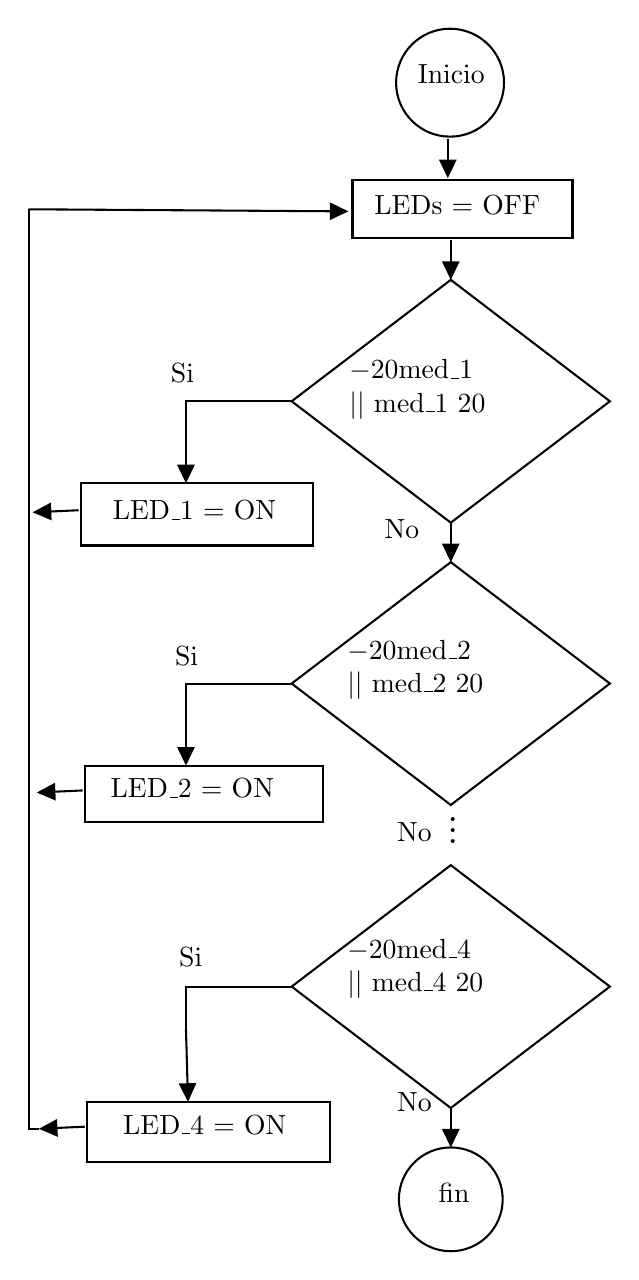
\begin{tikzpicture}[x=0.75pt,y=0.75pt,yscale=-1,xscale=1]
%uncomment if require: \path (0,689); %set diagram left start at 0, and has height of 689

%Flowchart: Connector [id:dp7813495520702245] 
\draw   (315,40) .. controls (315,25.64) and (326.64,14) .. (341,14) .. controls (355.36,14) and (367,25.64) .. (367,40) .. controls (367,54.36) and (355.36,66) .. (341,66) .. controls (326.64,66) and (315,54.36) .. (315,40) -- cycle ;
%Straight Lines [id:da8847526091998554] 
\draw    (339.92,67) -- (339.92,83) ;
\draw [shift={(339.92,86)}, rotate = 270] [fill={rgb, 255:red, 0; green, 0; blue, 0 }  ][line width=0.08]  [draw opacity=0] (8.93,-4.29) -- (0,0) -- (8.93,4.29) -- cycle    ;
%Flowchart: Decision [id:dp21596588394867888] 
\draw   (341.35,135) -- (418,193.5) -- (341.35,252) -- (264.69,193.5) -- cycle ;
%Straight Lines [id:da7204417446380422] 
\draw    (341.35,116) -- (341.35,132) ;
\draw [shift={(341.35,135)}, rotate = 270] [fill={rgb, 255:red, 0; green, 0; blue, 0 }  ][line width=0.08]  [draw opacity=0] (8.93,-4.29) -- (0,0) -- (8.93,4.29) -- cycle    ;
%Straight Lines [id:da49582350632228556] 
\draw    (213.76,214) -- (213.76,230) ;
\draw [shift={(213.76,233)}, rotate = 270] [fill={rgb, 255:red, 0; green, 0; blue, 0 }  ][line width=0.08]  [draw opacity=0] (8.93,-4.29) -- (0,0) -- (8.93,4.29) -- cycle    ;
%Straight Lines [id:da6050013822698619] 
\draw    (138,101) -- (289,101.98) ;
\draw [shift={(292,102)}, rotate = 180.37] [fill={rgb, 255:red, 0; green, 0; blue, 0 }  ][line width=0.08]  [draw opacity=0] (8.93,-4.29) -- (0,0) -- (8.93,4.29) -- cycle    ;
%Shape: Right Angle [id:dp2914826540765745] 
\draw   (264.69,193.5) -- (213.76,193.5) -- (213.76,214) ;
%Shape: Right Angle [id:dp7943090498770735] 
\draw   (142.92,544) -- (138,544) -- (138,101) ;
%Straight Lines [id:da15691850789793538] 
\draw    (162,246) -- (142.91,246.86) ;
\draw [shift={(139.92,247)}, rotate = 357.41] [fill={rgb, 255:red, 0; green, 0; blue, 0 }  ][line width=0.08]  [draw opacity=0] (8.93,-4.29) -- (0,0) -- (8.93,4.29) -- cycle    ;
%Flowchart: Process [id:dp025828036440153967] 
\draw   (163,233) -- (275,233) -- (275,263) -- (163,263) -- cycle ;
%Flowchart: Process [id:dp08317044111396199] 
\draw   (294,87) -- (400,87) -- (400,115) -- (294,115) -- cycle ;
%Flowchart: Decision [id:dp9588588712187942] 
\draw   (341.35,271) -- (418,329.5) -- (341.35,388) -- (264.69,329.5) -- cycle ;
%Straight Lines [id:da6075623967992321] 
\draw    (341.35,252) -- (341.35,268) ;
\draw [shift={(341.35,271)}, rotate = 270] [fill={rgb, 255:red, 0; green, 0; blue, 0 }  ][line width=0.08]  [draw opacity=0] (8.93,-4.29) -- (0,0) -- (8.93,4.29) -- cycle    ;
%Straight Lines [id:da7280821078053175] 
\draw    (213.76,350) -- (213.76,366) ;
\draw [shift={(213.76,369)}, rotate = 270] [fill={rgb, 255:red, 0; green, 0; blue, 0 }  ][line width=0.08]  [draw opacity=0] (8.93,-4.29) -- (0,0) -- (8.93,4.29) -- cycle    ;
%Shape: Right Angle [id:dp5301940302382446] 
\draw   (264.69,329.5) -- (213.76,329.5) -- (213.76,350) ;
%Flowchart: Process [id:dp03155186296961898] 
\draw   (165,369) -- (280,369) -- (280,396) -- (165,396) -- cycle ;
%Straight Lines [id:da8674623880313952] 
\draw    (164,381) -- (144.91,381.86) ;
\draw [shift={(141.92,382)}, rotate = 357.41] [fill={rgb, 255:red, 0; green, 0; blue, 0 }  ][line width=0.08]  [draw opacity=0] (8.93,-4.29) -- (0,0) -- (8.93,4.29) -- cycle    ;
%Flowchart: Decision [id:dp9506954994828107] 
\draw   (341.35,417) -- (418,475.5) -- (341.35,534) -- (264.69,475.5) -- cycle ;
%Straight Lines [id:da2567401210333511] 
\draw    (213.76,496) -- (214.67,528) ;
\draw [shift={(214.76,531)}, rotate = 268.36] [fill={rgb, 255:red, 0; green, 0; blue, 0 }  ][line width=0.08]  [draw opacity=0] (8.93,-4.29) -- (0,0) -- (8.93,4.29) -- cycle    ;
%Shape: Right Angle [id:dp7317557872750253] 
\draw   (264.69,475.5) -- (213.76,475.5) -- (213.76,496) ;
%Flowchart: Process [id:dp6148244624650872] 
\draw   (166,531) -- (283,531) -- (283,560) -- (166,560) -- cycle ;
%Straight Lines [id:da6248486907124713] 
\draw    (165,543) -- (145.91,543.86) ;
\draw [shift={(142.92,544)}, rotate = 357.41] [fill={rgb, 255:red, 0; green, 0; blue, 0 }  ][line width=0.08]  [draw opacity=0] (8.93,-4.29) -- (0,0) -- (8.93,4.29) -- cycle    ;
%Straight Lines [id:da1967066179049608] 
\draw    (341.35,534) -- (341.35,550) ;
\draw [shift={(341.35,553)}, rotate = 270] [fill={rgb, 255:red, 0; green, 0; blue, 0 }  ][line width=0.08]  [draw opacity=0] (8.93,-4.29) -- (0,0) -- (8.93,4.29) -- cycle    ;
%Shape: Circle [id:dp6512187196885593] 
\draw   (316.35,578) .. controls (316.35,564.19) and (327.54,553) .. (341.35,553) .. controls (355.15,553) and (366.35,564.19) .. (366.35,578) .. controls (366.35,591.81) and (355.15,603) .. (341.35,603) .. controls (327.54,603) and (316.35,591.81) .. (316.35,578) -- cycle ;

% Text Node
\draw (324,30) node [anchor=north west][inner sep=0.75pt]   [align=left] {Inicio};
% Text Node
\draw (291,172) node [anchor=north west][inner sep=0.75pt]   [align=left] {$\displaystyle -20\geqslant $med\_1 \\$\displaystyle ||$ med\_1 $\displaystyle \geqslant 20$};
% Text Node
\draw (308,249) node [anchor=north west][inner sep=0.75pt]   [align=left] {No};
% Text Node
\draw (205,174) node [anchor=north west][inner sep=0.75pt]   [align=left] {Si};
% Text Node
\draw (177,240) node [anchor=north west][inner sep=0.75pt]   [align=left] {LED\_1 = ON};
% Text Node
\draw (303,93) node [anchor=north west][inner sep=0.75pt]   [align=left] {LEDs = OFF};
% Text Node
\draw (290,307) node [anchor=north west][inner sep=0.75pt]   [align=left] {$\displaystyle -20\geqslant $med\_2 \\$\displaystyle ||$ med\_2 $\displaystyle \geqslant 20$};
% Text Node
\draw (207,310) node [anchor=north west][inner sep=0.75pt]   [align=left] {Si};
% Text Node
\draw (176,374) node [anchor=north west][inner sep=0.75pt]   [align=left] {LED\_2 = ON};
% Text Node
\draw (338,384.4) node [anchor=north west][inner sep=0.75pt]  [font=\LARGE]  {$\vdots $};
% Text Node
\draw (334,569) node [anchor=north west][inner sep=0.75pt]   [align=left] {fin};
% Text Node
\draw (290,451) node [anchor=north west][inner sep=0.75pt]   [align=left] {$\displaystyle -20\geqslant $med\_4 \\$\displaystyle ||$ med\_4 $\displaystyle \geqslant 20$};
% Text Node
\draw (209,455) node [anchor=north west][inner sep=0.75pt]   [align=left] {Si};
% Text Node
\draw (182,536) node [anchor=north west][inner sep=0.75pt]   [align=left] {LED\_4 = ON};
% Text Node
\draw (314,395) node [anchor=north west][inner sep=0.75pt]   [align=left] {No};
% Text Node
\draw (314,525) node [anchor=north west][inner sep=0.75pt]   [align=left] {No};


\end{tikzpicture}

\caption{Diagrama de flujo alarma AC/DC.}
\label{sch4}
\end{figure}